\documentclass[main.tex]{subfiles}

\begin{document}
We start by recalling the formula for the socle layers of the injective tensor $\mathfrak{sp}_\infty-$module $\Gamma_\lambda$.
\begin{thm}{\cite{penkov2007tensorrepresentationsclassicallocally}, \cite{dancohen2012koszulcategoryrepresentationsfinitary}}
\label{thm-soc}
    For any partition $\lambda$, the $\mathfrak{sp}_\infty-$module $\Gamma_\lambda$ is an injective hull of $\Gamma_{<\lambda>}$ and is hence indecomposable. The socle layers of $\Gamma_\lambda$ are given by
    $$
    \soc{k+1}\Gamma_\lambda = \bigoplus\limits_{\mu} \left( \sum\limits_{|\gamma|=k} \LR{\lambda}{\mu}{(2\gamma)^T} \right) \Gamma_{<\mu>}
    \hspace{0.7cm} \text{ for } k = 1, ..., \left[\frac{n}{2}\right], n = |\lambda|.$$
\end{thm}
\bigskip

\begin{ex}
    \label{ex-socle-filtration}
    The table below shows the socle layers of the $\mathfrak{sp}_\infty-$ module $\Gamma_{(3,2,1,1)}$: \\
    
    \begin{table}[H]
    \centering
    \begin{tabular}{|c|}
        \hline
        $\Gamma_{<(1)>}$ \\
        \hline $2\Gamma_{<(2,1)>} \oplus \Gamma_{<(1,1,1)>}$ \\
       \hline $\Gamma_{<(3,2)>} \oplus \Gamma_{<(2,2,1)>} \oplus \Gamma_{<(2,1,1,1)>} \oplus \Gamma_{<(3,1,1)>}$ \\
        \hline $\Gamma_{<(3,2,1,1)>}$ \\
        \hline
    \end{tabular}
\end{table}
In more detail: the degree of $(3,2,1,1)$ is $7$, so according to Theorem \ref{thm-soc} we can have at most $1+\left[\frac{7}{2}\right]=4$ socle layers. We know from section 2 of the thesis that $\soc{1}\Gamma_{(3,2,1,1)} = soc\;\Gamma_{(3,2,1,1)} = \Gamma_{<(3,2,1,1)>}$. In the second layer we need to use a  degree 2 partition of the form $(2\gamma)^T$, and the only one is $(1,1).$ We are interested in finding the subpartitions $\mu$ of $(3,2,1,1)$ for which there exists at least one Littlewood-Richardson tableau of shape $(3,2,1,1)/(1,1)$ and weight $\mu$. The only possible such subpartitions are $(3,2), (2,2,1), (2,1,1,1), (3,1,1),$ and the second socle layer is: 
$$
    \soc{2}\Gamma_{(3,2,1,1)} =  \LR{(3,2,1,1)}{(3,2)}{(1,1)} \Gamma_{<(3,2)>}\oplus \LR{(3,2,1,1)}{(2,2,1)}{(1,1)} \Gamma_{<(2,2,1)>} \oplus
    \LR{(3,2,1,1)}{(2,1,1,1)}{(1,1)} \Gamma_{<(2,1,1,1)>}\oplus
    \LR{(3,2,1,1)}{(3,1,1)}{(1,1)} \Gamma_{<(3,1,1)>}=
$$
$$
    = \Gamma_{<(3,2)>}\oplus \Gamma_{<(2,2,1)>} \oplus \Gamma_{<(2,1,1,1)>}\oplus \Gamma_{<(3,1,1)>}.
$$
The next two socle layers are computed in a similar fashion:
$$
    \soc{3}\Gamma_{(3,2,1,1)} =  \LR{(3,2,1,1)}{(2,1)}{(2,2)} \Gamma_{<(2,1)>}\oplus \LR{(3,2,1,1)}{(2,2)}{(1,1,1)} \Gamma_{<(1,1,1)>} \oplus
    \LR{(3,2,1,1)}{(1,1,1,1)}{(3,2,1,1)} \Gamma_{<(2,1)>}= 2\Gamma_{<(2,1)>}\oplus\Gamma_{<(1,1,1)>},
$$
$$
    \soc{4}\Gamma_{(3,2,1,1)} =  \LR{(3,2,1,1)}{(2,2,1,1)}{(1)} \Gamma_{<(1)>} = \Gamma_{<(1)>}.
$$
\end{ex}
\bigskip

Theorem \ref{thm-soc} computes the length of the socle filtration of the injective tensor module $\Gamma_\lambda$ only implicitly. Our first result in this thesis is the following explicit formula (proposition \ref{socle-filtr-height}) for the length of this socle filtration.  For this, we introduce the notion of \textbf{even degree} of a partition. 
\bigskip

\begin{defn}[\textbf{Even degree of a partition}]
    Given a partition $\lambda = (\lambda_1,\lambda_2, ..., \lambda_r)$, let $|\lambda|^{even}$ denote the sum of the entries on even positions $\lambda_2, \lambda_4, \lambda_6, ...$, and call it the \textbf{even degree} of $\lambda$. 
\end{defn}

\bigskip
The following is our first result:
\begin{prop}
    \label{socle-filtr-height}
    For any partition $\lambda$, the last nonzero socle layer in the socle filtration of the $\mathfrak{sp}_\infty$-module $\Gamma_\lambda$ is:
    $$
    \soc{k+1}\Gamma_\lambda = \bigoplus\limits_{\mu} \left( \sum\limits_{|\gamma|=k} \LR{\lambda}{\mu}{(2\gamma)^T} \right) \Gamma_{<\mu>}
    \hspace{0.7cm} \text{ for } k = |\lambda|^{even}.
    $$
    Moreover, the module $\Gamma_{<(s)>}$ with $s = |\lambda| - 2|\lambda|^{even}$ is always a simple constituent of the last nonzero socle layer and appears with multiplicity one.
\end{prop}
\begin{proof}
    We divide the proof into two steps: showing that $\soc{k+1}\Gamma_\lambda$  is indeed nonzero for $k=|\lambda|^{even}$, and proving that $\soc{k+1}\Gamma_\lambda=0$ for any $k>|\lambda|^{even}.$ For both steps we need to find the maximal $(2\gamma)^T$ subpartition of $\lambda = (\lambda_1, \lambda_2, ..., \lambda_r).$  \\

    Let $r=2m$ or $r=2m+1$ for some positive integer $m.$ Then the even degree of $\lambda$ is $|\lambda|^{even} = \lambda_2+\lambda_4+...+\lambda_{2m}$. We claim that the unique maximal subpartition of $\lambda$ of type $(2\gamma)^T$ has degree $2|\lambda|^{even}$ and is $$(2\gamma)^T_{max}:=(\lambda_2, \lambda_2, \lambda_4, \lambda_4, ..., \lambda_{2m}, \lambda_{2m}).$$ 

    We first show the maximality and uniqueness of the partition $(2\gamma)^T_{max}$.
    Suppose that $\eta=(2\gamma)^T$  is a subpartition of $\lambda$, for some partition $\gamma$. Then $\eta$ has even length $2p$ and $\eta_{2i-1}=\eta_{2i}\leq \lambda_{2i}$ for any $i\leq min(m,p)$. Thus 
    $$
    |\eta|=2\sum\limits_{i=1}^{min(m,p)}\eta_{2i}\leq 2\sum\limits_{i=1}^{m}\lambda_{2i} = 2|\lambda|^{even}. 
    $$
    Equality holds only when all inequalities $\eta_{2i-1}=\eta_{2i}\leq \lambda_{2i}$ are equalities and $m=p$. Therefore, $\eta_{2i-1}=\eta_{2i}=\lambda_{2i}$ for $1\leq i\leq m$ is the only situation which leads to a subpartition of the form $(2\gamma)^T$ of $\lambda$ of maximal degree, hence $(2\gamma)^T_{max}=(\lambda_2, \lambda_2, \lambda_4, \lambda_4, ..., \lambda_{2m}, \lambda_{2m})$ is indeed the only such subpartition of $\lambda$.\\

    Since $(2\gamma)^T_{max}$ has degree $2|\lambda|^{even},$ we conclude that $\LR{\lambda}{\mu}{(2\gamma)^T}=0$ for any partition $\mu$ of degree less than $|\lambda|-2|\lambda|^{even}$, i.e. that
    any $(k+1)^{th}$ socle layer of $\Gamma_\lambda$ is zero for $k>|\lambda|^{even}$.\\  

    Next, we need to prove that $\soc{k+1}\Gamma_\lambda = \bigoplus\limits_{\mu} \left( \sum\limits_{|\gamma|=k} \LR{\lambda}{\mu}{(2\gamma)^T} \right) \Gamma_{<\mu>} 
   $ is nonzero for $ k = |\lambda|^{even}.$ For this, we only need to show the existence of a partition $\mu$ for which $\LR{\lambda}{\mu}{(2\gamma)^T_{max}}>0$. 
  We take $\mu$ to be the row-partition $(s)$ for $s := |\lambda|-2\cdot |\lambda|^{even} = |\lambda| - |{(2\gamma)^T_{max}}|.$ Then we can conclude from Pieri's rule on Young diagrams that  $\LR{\lambda}{(s)}{(2\gamma)^T_{max}}=1,$ since we are attaching the boxes from $\mu$ only on the odd-numbered rows of the Young diagram with no overlap on the columns. This means that $\Gamma_{<(s)>}$ appears in the top layer of the socle filtration with multiplicity $1$.\\

\end{proof}

\bigskip


We now prove a stronger result concerning the last socle layer of $\Gamma_\lambda.$\\
\bigskip

\begin{prop}
\label{prop-soc-last-term-general}
     Let $\lambda = (\lambda_1, \lambda_2, ..., \lambda_{r})$ be a partition. If $r=2m$ for some positive integer $m,$ we pick the nonzero values among the set of differences $\{\lambda_1-\lambda_2, \lambda_3-\lambda_4, ..., \lambda_{2m-1}-\lambda_{2m}\}.$ If $r=2m+1$ for some positive integer $m$, we pick the nonzero values from $\{\lambda_1-\lambda_2, \lambda_3-\lambda_4, ..., \lambda_{2m-1}-\lambda_{2m}, \lambda_{2m+1}\}.$ Rearranging these nonzero values in a descending order, we obtain a partition $(y_1, y_2, ..., y_l)$. 
     Then for any partition $\mu$ with $\mu\geq_{lex}(y_1, y_2, ..., y_l), \; |\mu|=|(y_1, y_2, ..., y_l)|$, and of length at most $l$, the simple $\mathfrak{sp}_\infty-$module $\Gamma_{<\mu>}$ appears in the last term of the socle filtration of  $\Gamma_\lambda$. 
\end{prop}

\begin{proof}
    The case where $\mu = (\sum\limits_{i=1}^{l}y_i)$ is described in the last proposition. For the general case, we need to show that we can find at least one Littlewood-Richardson tableau of size $\lambda/{(2\gamma)^T}_{max}$ and of weight $\mu = (\mu_1, \mu_2, ..., \mu_t)\geq_{lex} (y_1, y_2, ..., y_l),\; t\leq l$. The skew diagram of size $\lambda/{(2\gamma)^T}_{max}$ contains only columns of length $1,$ so the Littlewood-Richardson rule is easier to check.  \\

   We construct such a Littlewood-Richardson tableau of size $\lambda/{(2\gamma)^T}_{\text{max}}$ and of weight $(\mu_1, \mu_2,..., \mu_t)$ by placing the numbers $\underbrace{1,1,...,1}_{\mu_1 \text{ times }}, \underbrace{2,2,...,2}_{\mu_2 \text{ times }}, ..., \underbrace{t,t,...,t}_{\mu_t \text{ times}}$  in a step-by-step manner. In the procedure we describe below, we count the rows from the bottom row to the top row of the skew diagram, and say that a row is \textit{incomplete} if it has at least one box with no number written inside it.

    \begin{enumerate}
        \item This is a recursive procedure. In the rightmost empty box of the first incomplete row, we write the greatest number $x$ from the unplaced numbers of the multiset $\underbrace{1,1,...,1}_{\mu_1 \text{ times }}, \underbrace{2,2,...,2}_{\mu_2 \text{ times }}, ..., \underbrace{t,t,...,t}_{\mu_t \text{ times}}$ corresponding to the weight $\mu$. In the rightmost empty box from the next incomplete row above,  we write $x-1$, and so on until placing $1$. We repeat this step until all the boxes of the tableau are filled. Note that the total number of steps we need to place all numbers is $\mu_1$, and the number $i\in\{1,2,...,t\}$ is fully placed in the boxes of the tableau exactly when performing the first $\mu_i$ steps.

        \item After all numbers are placed, some rows may may not be monotonous. We rearrange the boxes of those rows so that each row's entries are in a non-strict increasing order from left to right.

    \end{enumerate}

    After applying this algorithm, one can immediately observe that the equivalent conditions from definitions \ref{def-partition-expansion} and \ref{def-skew-tableau} are satisfied, and the statement follows.

\end{proof}
\bigskip

We conjecture that, apart from the modules described in the proposition above, there are no other modules in the last socle layer. While we do not have a proof for this, it is confirmed by multiple examples done via programming.\\

\bigskip

\begin{ex}
\label{ex-algorithm-tableau}
    Let us use the step-by-step construction described in the proof of Proposition \ref{prop-soc-last-term-general} to fill in the boxes of the skew diagram of shape $(18, 16, 16, 12, 12, 10, 10, 4, 4)/(16,16,12,12,10,10,4,4)$, where the partition of nonzero differences is $(6,4,4,2,2)$. We will look at a particular example of  tableau with weight given by partition $\mu =(10,6,2) \geq_{lex}(6,4,4,2,2)$. The length of the partition $\mu$  is $3,$ so the boxes will only contain the numbers $1, 2,$ and $3$.\\
    
    Recall that we are counting the rows from the bottom row to the top row. Applying step 1 for the first time, we place 3 in the rightmost box of the first (lowest) row, then we place 2 in the rightmost box of the row above, and 1 in the rightmost box of the third row. Then, we repeat the process with the rightmost free boxes of these incomplete rows. Note that we are done placing the number $3$, after exactly $\mu_3=2$ algorithm steps, as in figure \ref{fig:tableaux-step1}.\\

    \begin{figure}[H]
        \centering
        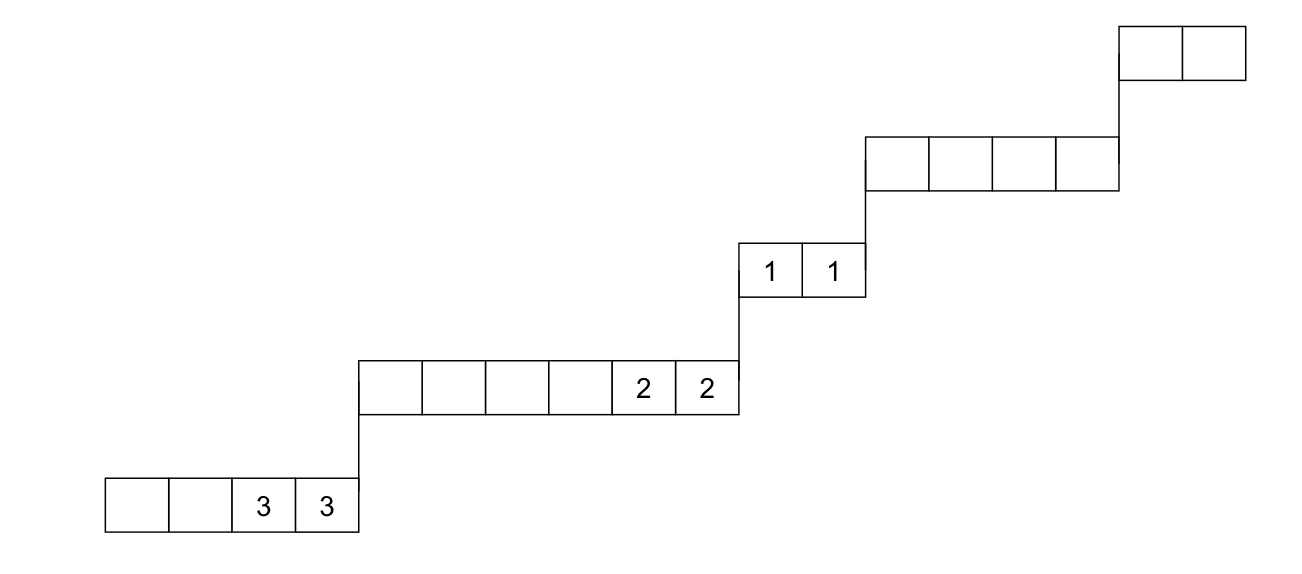
\includegraphics[width=0.6\linewidth]{images/tabl-step1.png}
        \caption{}
        \label{fig:tableaux-step1}
    \end{figure}

    Next, we consider the remaining empty boxes and start writing the unplaced numbers $$\underbrace{1,...,1}_{\mu_1-\mu_3=8 \text{ times }}, \underbrace{2,...,2}_{\mu_2-\mu_3=4 \text{ times }}.$$ In the next two steps,  we place $2$ twice in the first incomplete row, and $1$ twice in the row above. The row where 2 was placed now has no more empty boxes. The next two steps place the last appearances of $2$ in the boxes of the new first incomplete row (here, row 2) - its entries end up being 2,2,1,1,2,2, making the row non-increasing. The two placements of the number $1$ which correspond to the last $2$ entries will be in the boxes from the above incomplete row (here, row 4). These last 4 steps can be understood through the figure below.\\
    \begin{figure}[H]
        \centering
        \label{fig:tableaux-step2}
        \subfloat{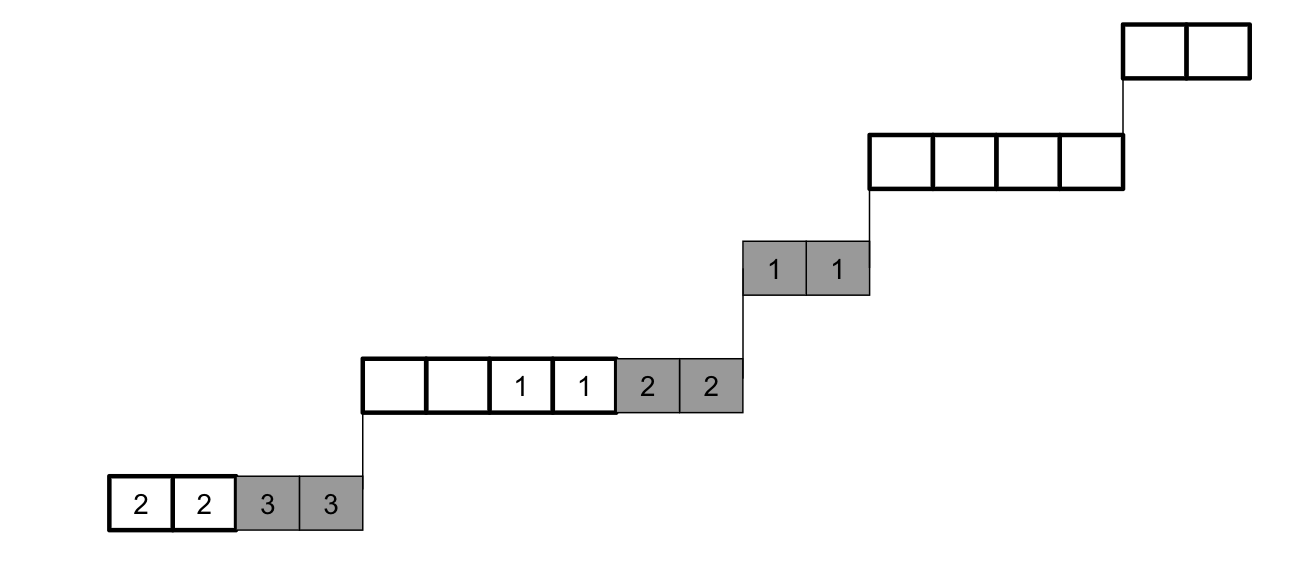
\includegraphics[width=0.5\linewidth]{images/tabl-step2-1.png}}
        \subfloat{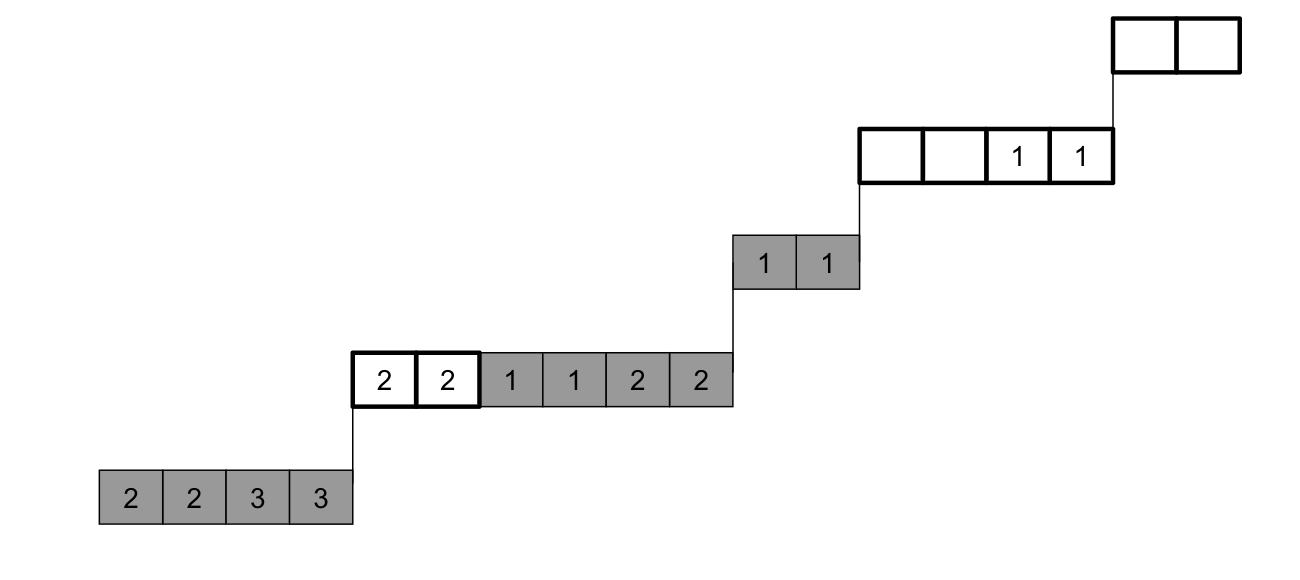
\includegraphics[width=0.5\linewidth]{images/tabl-step2-2.png}}

        \caption{}
    \end{figure}

    After this, we have to place $1$ in the remaining four boxes. We rearrange the boxes of the non-monotonous row of the tableau such that they are in an ascending order, and obtain the desired Littlewood-Richardson tableau.\\
    
    \begin{figure}[H]
        \centering
        \label{fig:tableaux-step3}
        \subfloat{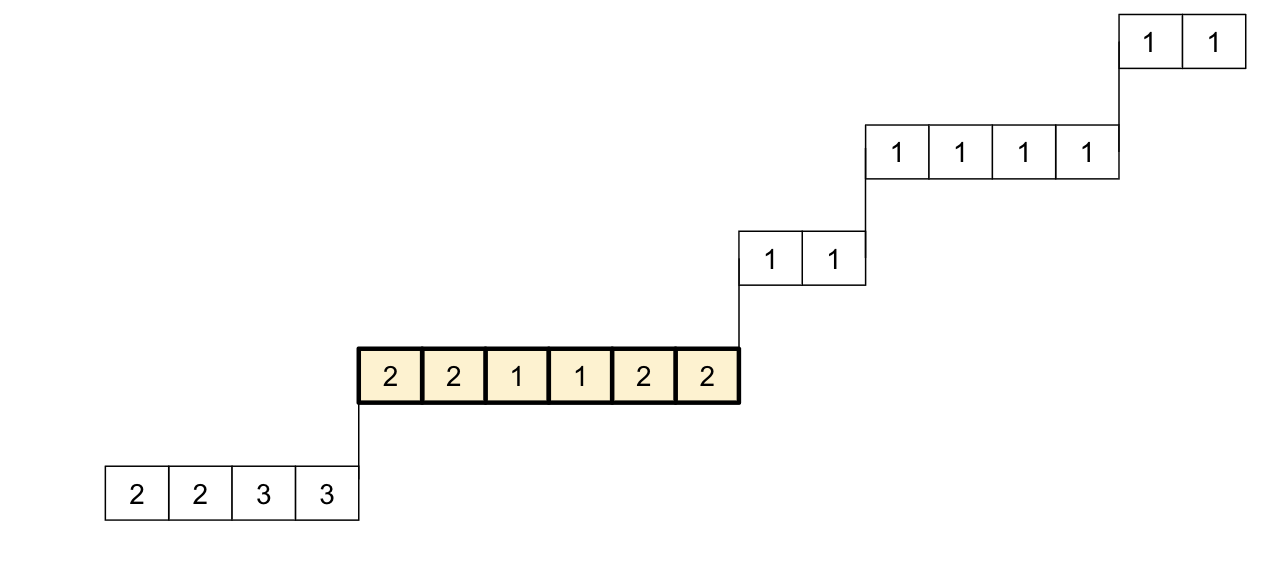
\includegraphics[width=0.5\linewidth]{images/tabl-step3.png}}
        \subfloat{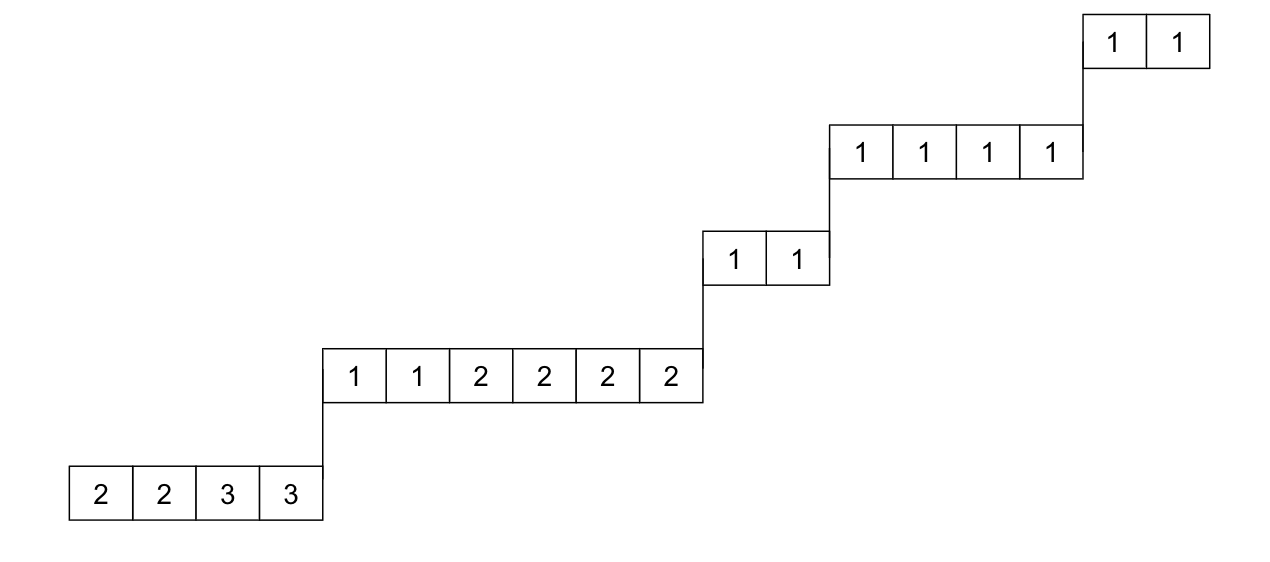
\includegraphics[width=0.5\linewidth]{images/tabl-final.png}}
        \caption{}
    \end{figure}

    One can see that, even with the rearrangement of the entries of a row, the strict $\mu-$expansion rule is still satisfied, as each number has all its predecessors written in upper rows. This shows that counting any set of boxes (from top to bottom, right to left), 1 appears at least as many times as 2 and 2 appears at least as many times as 3.  The property is emphasized in the colour-coordinated figure below.
    
    \begin{figure}[H]
        \centering
        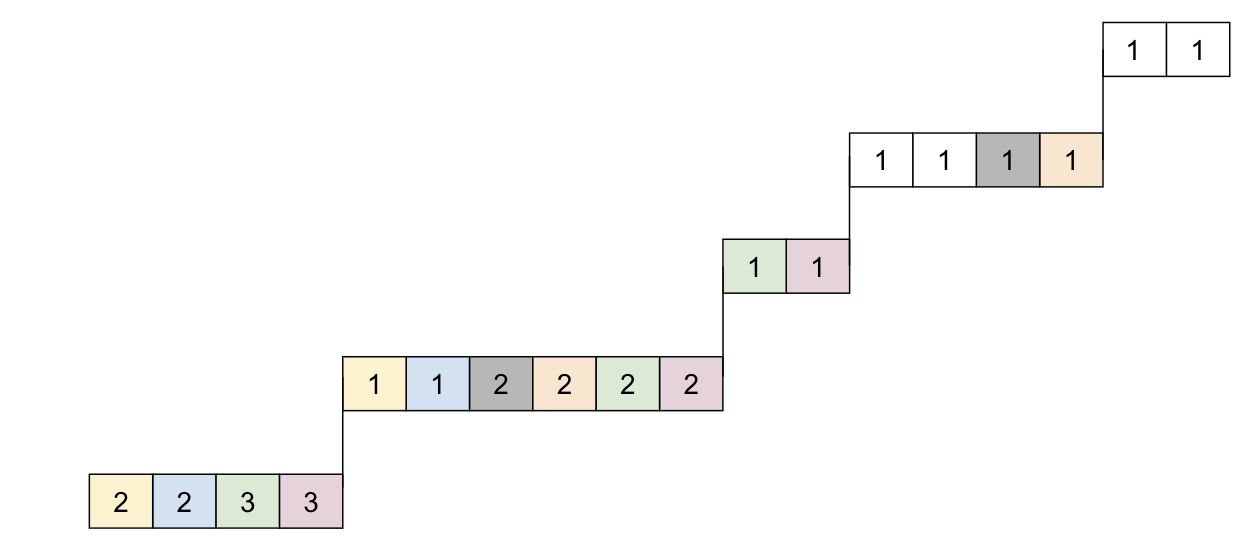
\includegraphics[width=0.5\linewidth]{images/tabl-colour.png}
        \label{fig:tableaux-colour}
        \caption{}
    \end{figure}    
\end{ex}
\bigskip

\begin{crl}
    For any partition $\lambda$, the trivial representation $\Gamma_{<\emptyset>}$ is a simple constituent of the last nonzero socle layer in the socle filtration of the $\mathfrak{sp}_\infty$-module $\Gamma_\lambda$ if and only if $\lambda = (2\gamma)^T$ for some partition $\gamma$.
    Furthermore, $\Gamma_{<\emptyset>}$ is the only term in the last socle layer of $\Gamma_\lambda$ and appears with multiplicity 1.
\end{crl}
\begin{proof}
    Straightforward.
\end{proof}

\bigskip

\begin{crl}
    Let $\lambda$ be a partition such that the partition of nonzero differences as defined in Proposition \ref{prop-soc-last-term-general} has length one, i.e. has the form $(y_1)$. Then the last nonzero socle layer in the socle filtration of the $\mathfrak{sp}_\infty$-module $\Gamma_\lambda$ equals $\Gamma_{<(y_1)>}$. Moreover, these modules $\Gamma_\lambda$ are the only ones with simple last socle layer.
\end{crl}
\begin{proof}
    Let $(2\gamma)^T_{max}$ be the unique maximal subpartition of $\lambda$ of form $(2\gamma)^T$. Then the semistandard skew tableau of shape $\lambda/(2\gamma)^T_{max}$ will be a row with $y_1$ boxes. The only Littlewood-Richardson tableau of this shape is the one with weight $(y_1)$, and $\LR{\lambda}{(2\gamma)^T_{max}}{(y_1)}=1$ by Pieri's rule on Young diagrams. So, $\Gamma_{<(y_1)>}$ appears in the last socle layer of the socle filtration of $\Gamma_\lambda$ with multiplicity 1.\\
    
    Suppose there exists a partition $\eta$ such that the partition of nonzero differences $(y_1',y_2',...,y_l')$, defined as in Proposition \ref{prop-soc-last-term-general}, has length at least $2.$ Then from the same proposition, we know that $\Gamma_{<(y_1',y_2',...,y_l')>}$ appears in the last socle layer. By Proposition \ref{socle-filtr-height}, $\Gamma_{<(y_1'+y_2'+...+y_l')>}$ is a simple constituent of the last socle layer too, and $\Gamma_{<(y_1',y_2',...,y_l')>}$ and $\Gamma_{<(y_1'+y_2'+...+y_l')>}$ are nonisomorphic. Therefore, if the partition of nonzero differences has length strictly greater than $1,$ then the last layer of the socle filtration of $\Gamma_{\eta}$ has at least two direct summands.
\end{proof}
\end{document}